\documentclass[11pt]{article}

\usepackage{amsmath}
\usepackage{graphicx}
\usepackage{subcaption}

\newcommand{\numpy}{{\tt numpy}}    % tt font for numpy

\topmargin -.5in
\textheight 9in
\oddsidemargin -.25in
\evensidemargin -.25in
\textwidth 7in

\begin{document}

% ========== Edit your name here
\author{Aobo Yang (ay6gv)}
\title{CS6316: HW2}
\maketitle

\medskip

% ========== Begin answering questions here
\begin{enumerate}

\item
Polynomial Regression

1.1 Data Generation

\medskip

The generated data distribution is shown in Figure \ref{fig:data}.

\begin{figure}[!h]
  \centering
  \begin{subfigure}[b]{0.4\linewidth}
    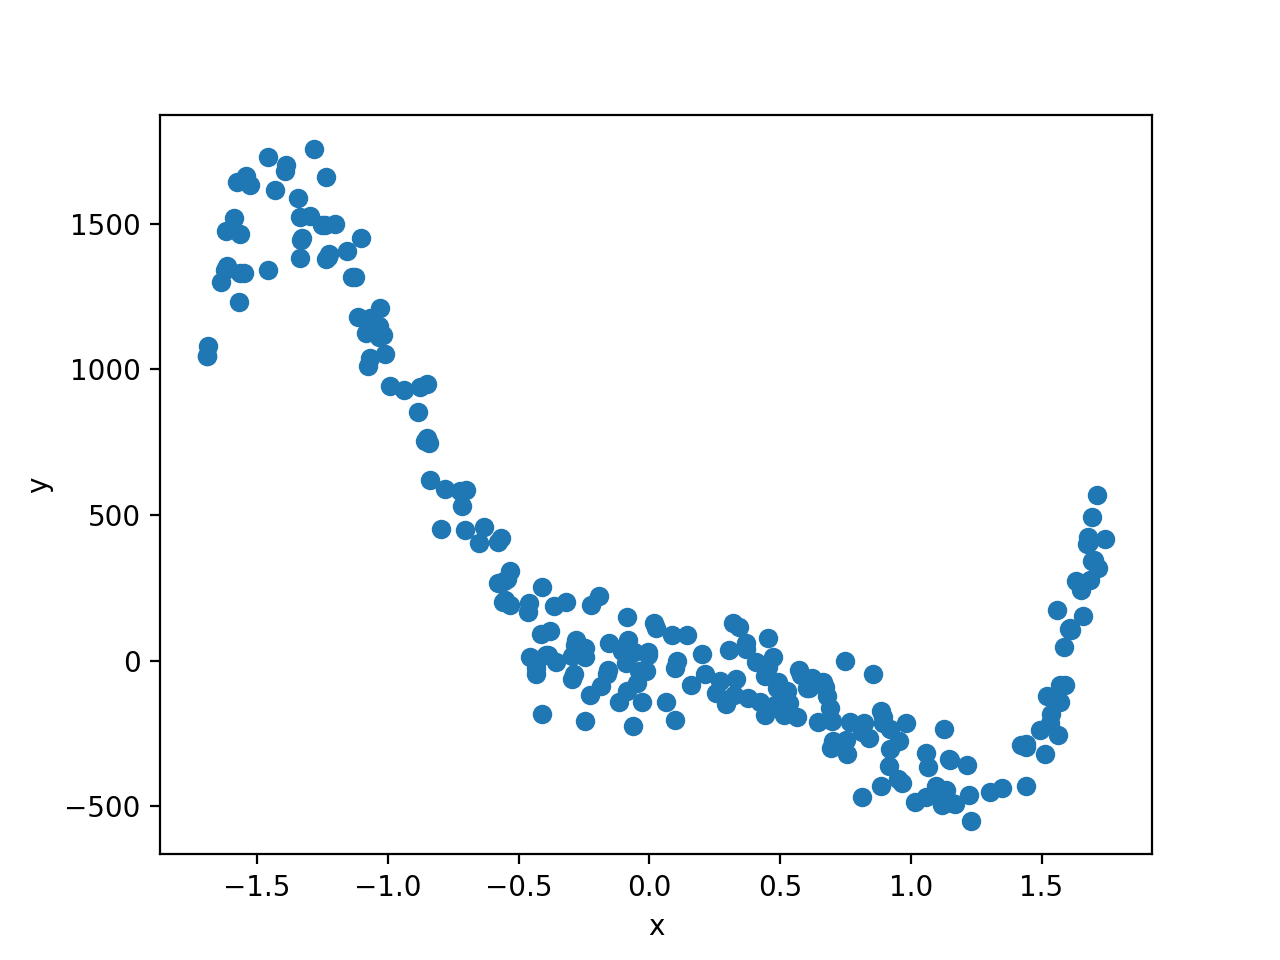
\includegraphics[width=\linewidth]{figures/data_train.png}
    \caption{Training}
  \end{subfigure}
  \begin{subfigure}[b]{0.4\linewidth}
    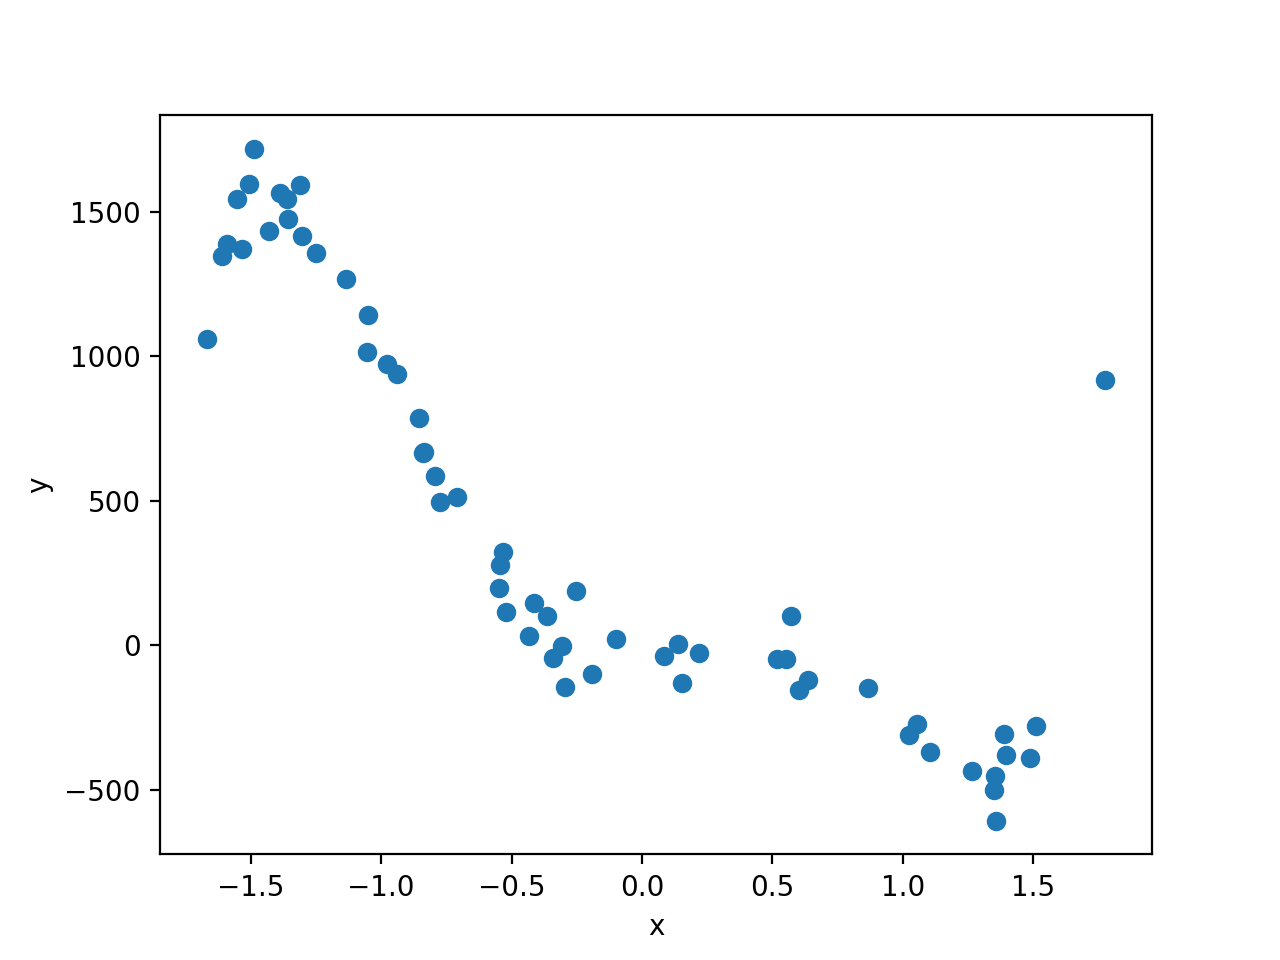
\includegraphics[width=\linewidth]{figures/data_test.png}
    \caption{Testing}
  \end{subfigure}
  \caption{Gradient Descent}
  \label{fig:data}
\end{figure}


1.2 Polynomial Regression Model Fitting

\medskip

The training and validation losses of different polynomial degrees is shown in Figure \ref{fig:poly_order_loss}. The best hyperparamter degree $d$ is $7$.


\begin{figure}[!h]
  \centering
  \begin{subfigure}[b]{0.4\linewidth}
    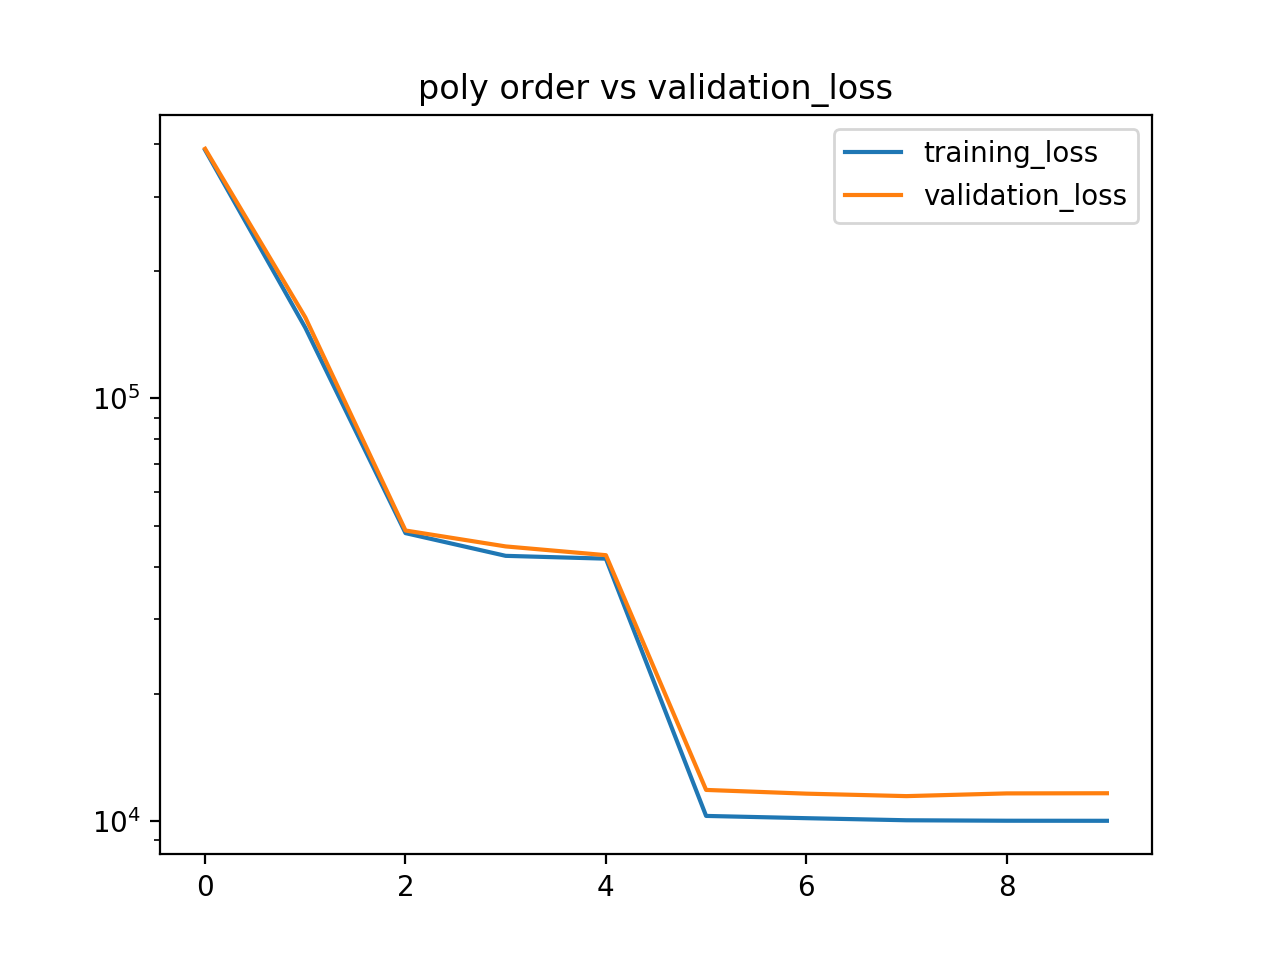
\includegraphics[width=\linewidth]{figures/poly_order_loss.png}
  \end{subfigure}
  \caption{Loss of Polynomial Orders}
  \label{fig:poly_order_loss}
\end{figure}

\medskip

The best $\Theta$ learned is $[-29.60722754,\, -13.93265366,\, 366.49596123,\, -1100.45557026,\, 23.79149025,\,$

$432.79168423,\, -20.91996714,\, -25.45551777]$, which sequentially act as the coefficients of order $0$ to $7$. The testing MSE loss is $8770.13$. The curve is shown in Figure \ref{fig:best_ne}. As required, the best $\Theta$ is gotten in two steps. First, the training data is futher split into training and validation to find the best polynomial order. Second, merge validation back to training and use the whole with normal equation to get this $\Theta$. Comparing with the numbers in data generation, our leaned $\Theta$ is actually reasonable. Although the absolute value scale is quite different, it is because the data has been normalized in data generation. Considering the sign and relative value scale, the learned $\Theta$ matches the data generation. For example, the values for order $6$ and $7$ are negligible, which do not exist in the original data generation.

\begin{figure}[!h]
  \centering
  \begin{subfigure}[b]{0.4\linewidth}
    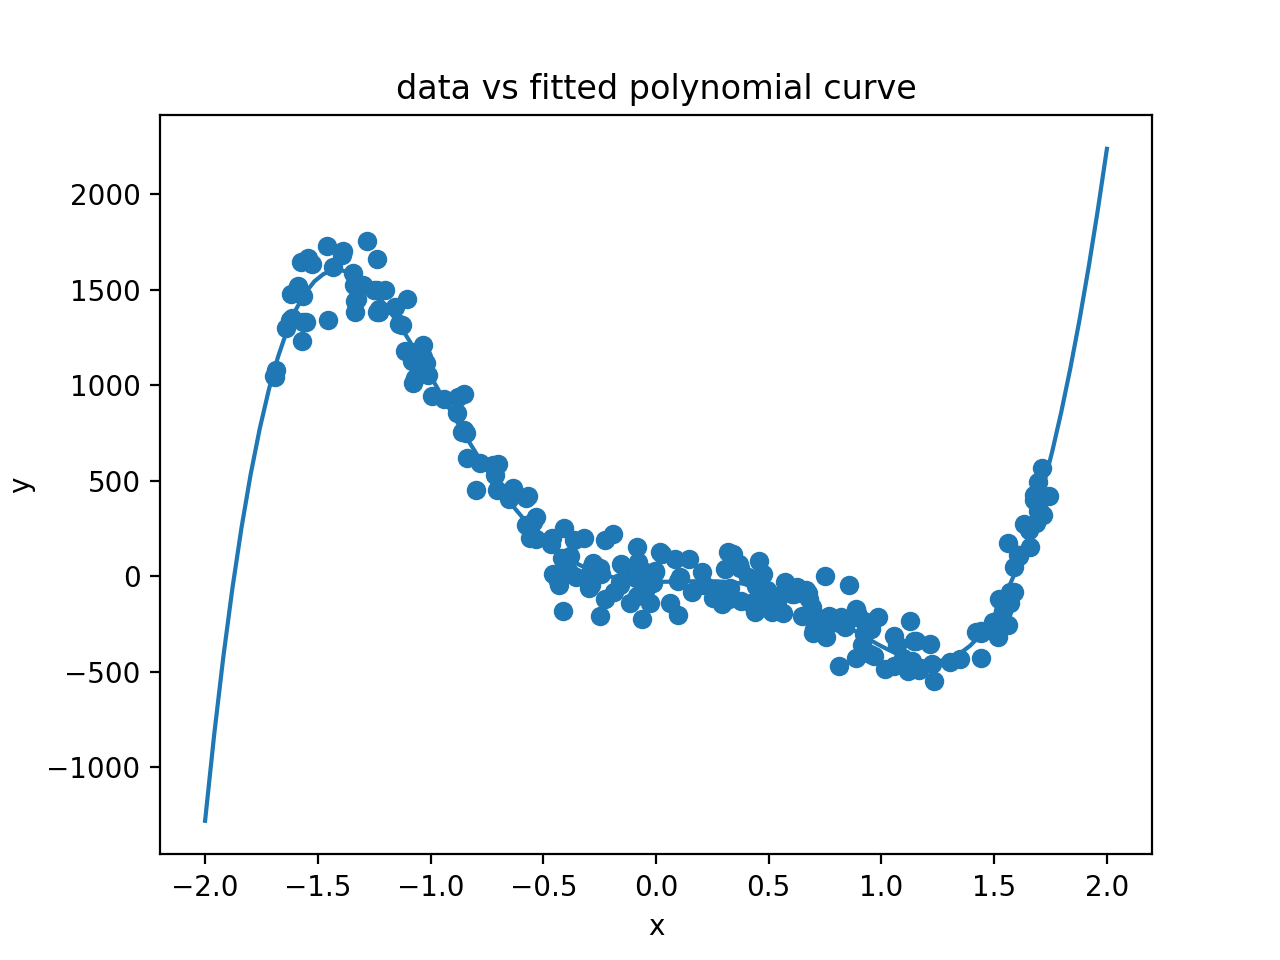
\includegraphics[width=\linewidth]{figures/best_ne_train.png}
    \caption{Training Data}
  \end{subfigure}
  \begin{subfigure}[b]{0.4\linewidth}
    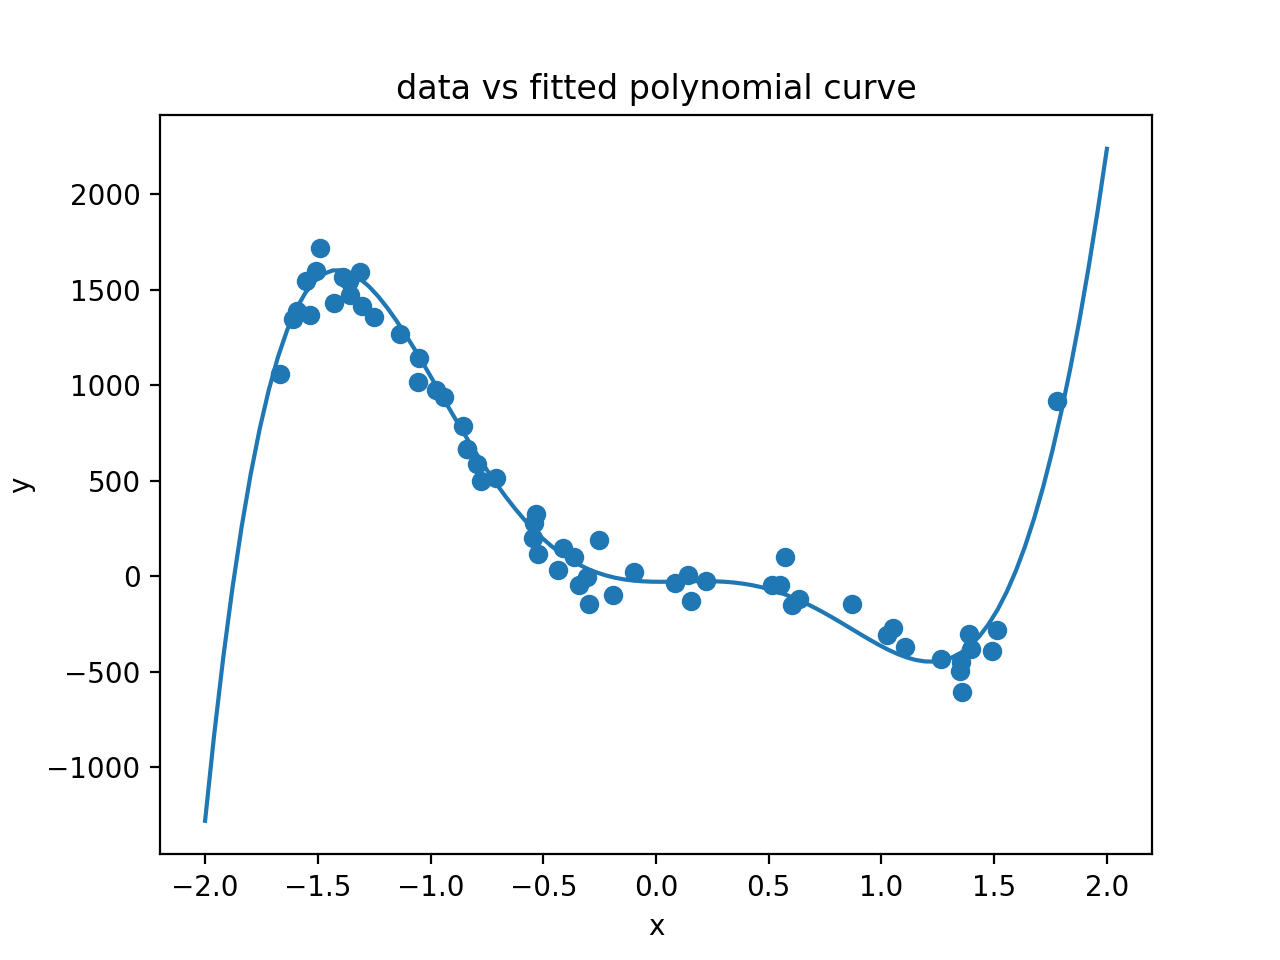
\includegraphics[width=\linewidth]{figures/best_ne_test.png}
    \caption{Testing Data}
  \end{subfigure}
  \caption{Learned Curve}
  \label{fig:best_ne}
\end{figure}

Keeping the degree as $7$, the learned curve and corresponding epoch losses are shown in Firgure \ref{fig:gd_7}. The same plots for degree $2$ is shown in Firgure \ref{fig:gd_2}. The model curve of degree $7$ is much more complex and the end loss is obviously lower then degree $2$. The training loss is lower than validation loss in degree $7$, but in degree $2$, the training loss is even higher. It means the model is too simple and cannot fit the data.

\begin{figure}[!h]
  \centering
  \begin{subfigure}[b]{0.4\linewidth}
    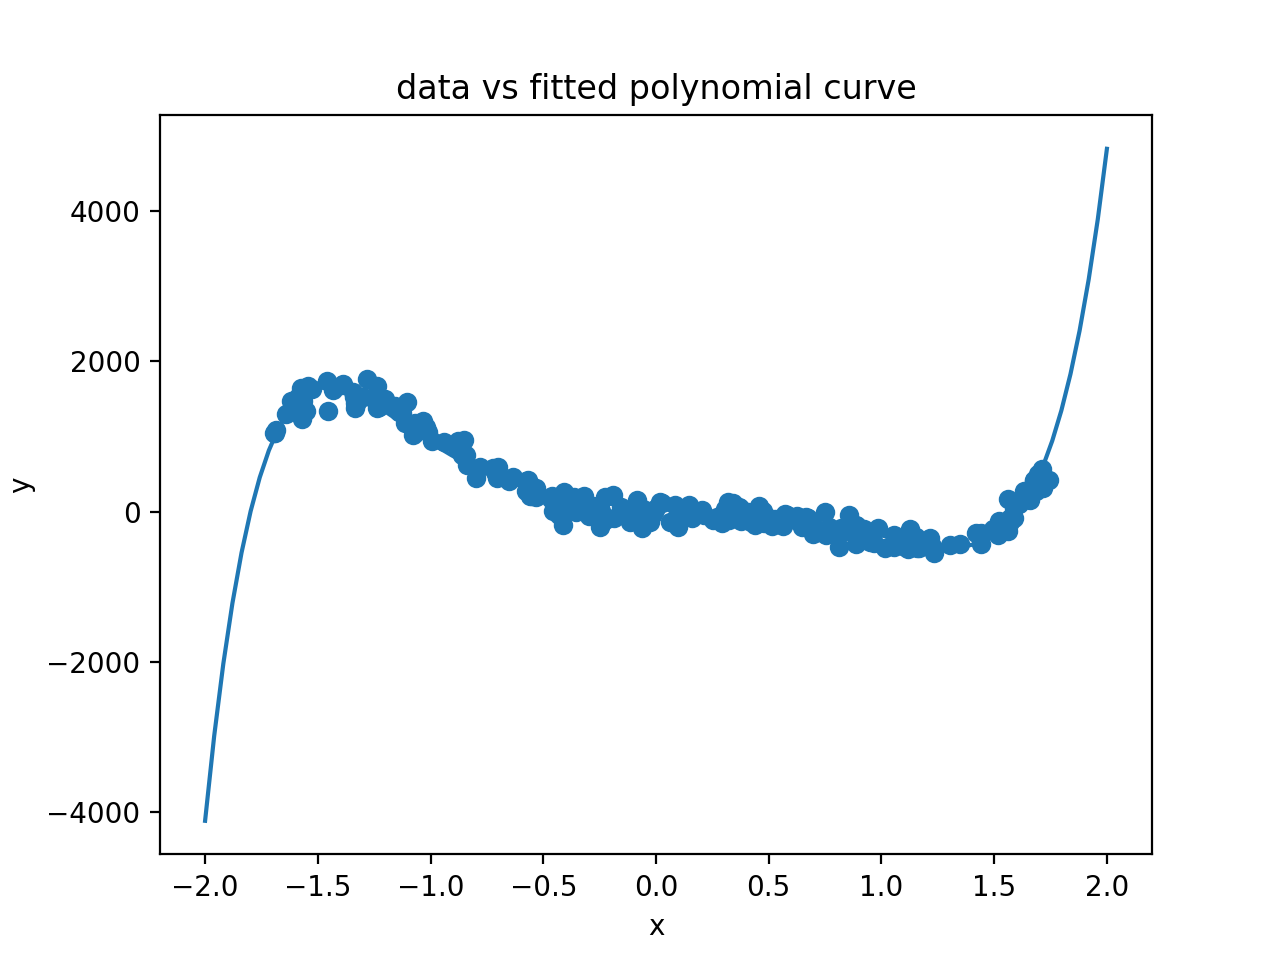
\includegraphics[width=\linewidth]{figures/best_gd_train.png}
    \caption{Training Data}
  \end{subfigure}
  \begin{subfigure}[b]{0.4\linewidth}
    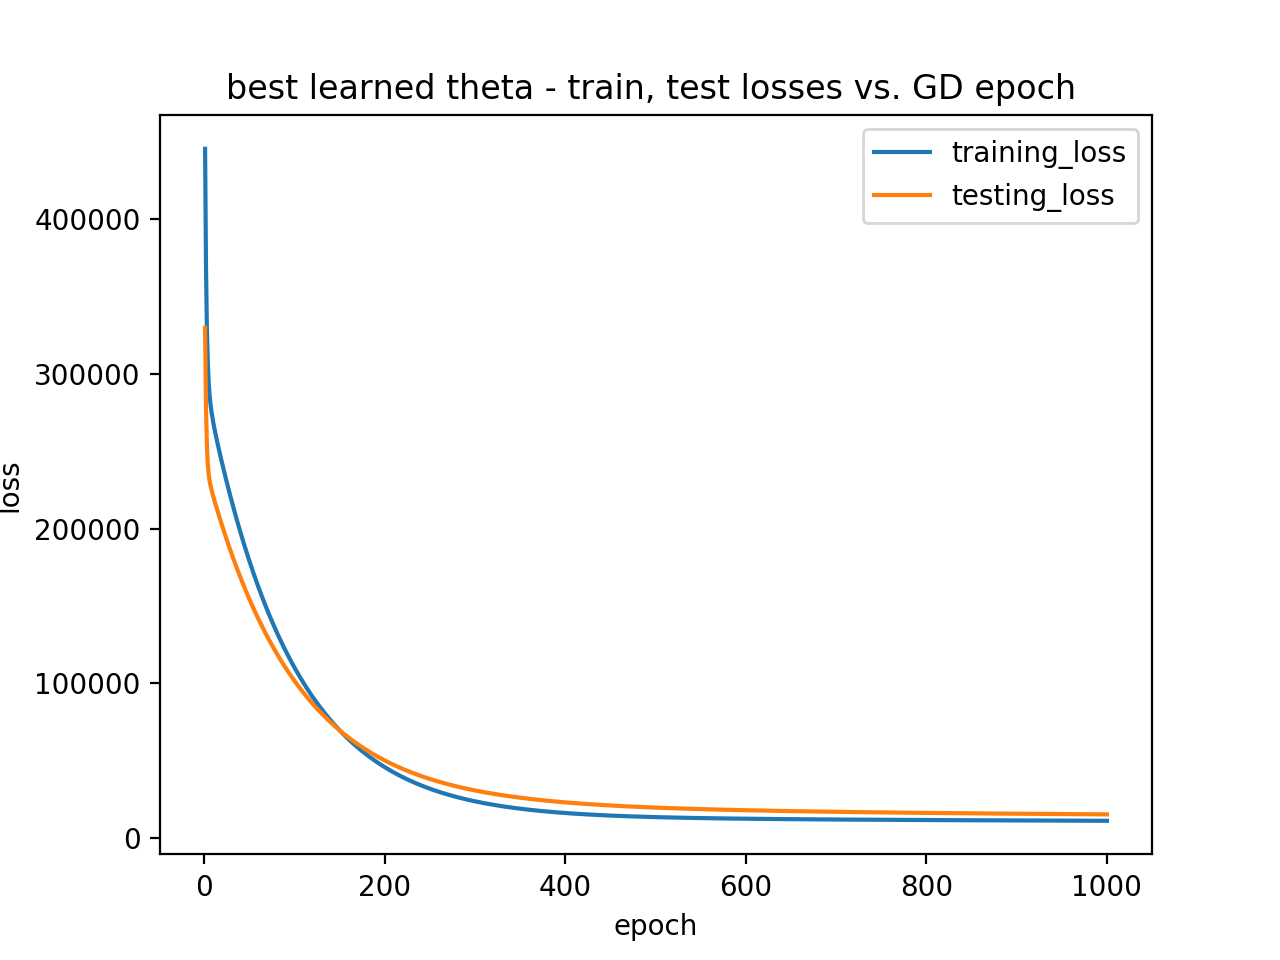
\includegraphics[width=\linewidth]{figures/best_gd_loss.png}
    \caption{Training \& Testing Loss}
  \end{subfigure}
  \caption{Gradient Descent with Degree 7}
  \label{fig:gd_7}
\end{figure}


\begin{figure}[!h]
  \centering
  \begin{subfigure}[b]{0.4\linewidth}
    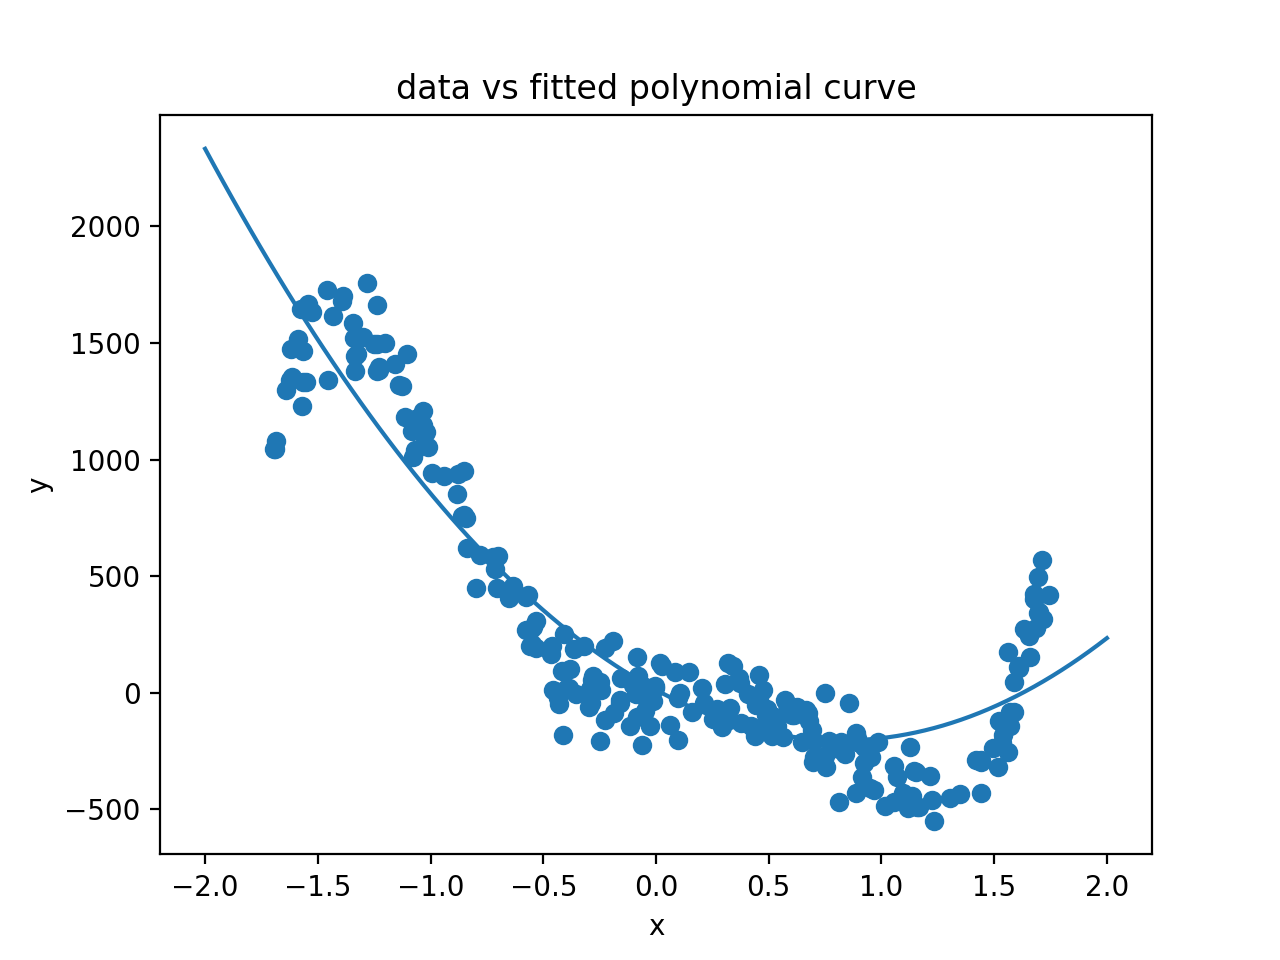
\includegraphics[width=\linewidth]{figures/d2_gd_train.png}
    \caption{Training Data}
  \end{subfigure}
  \begin{subfigure}[b]{0.4\linewidth}
    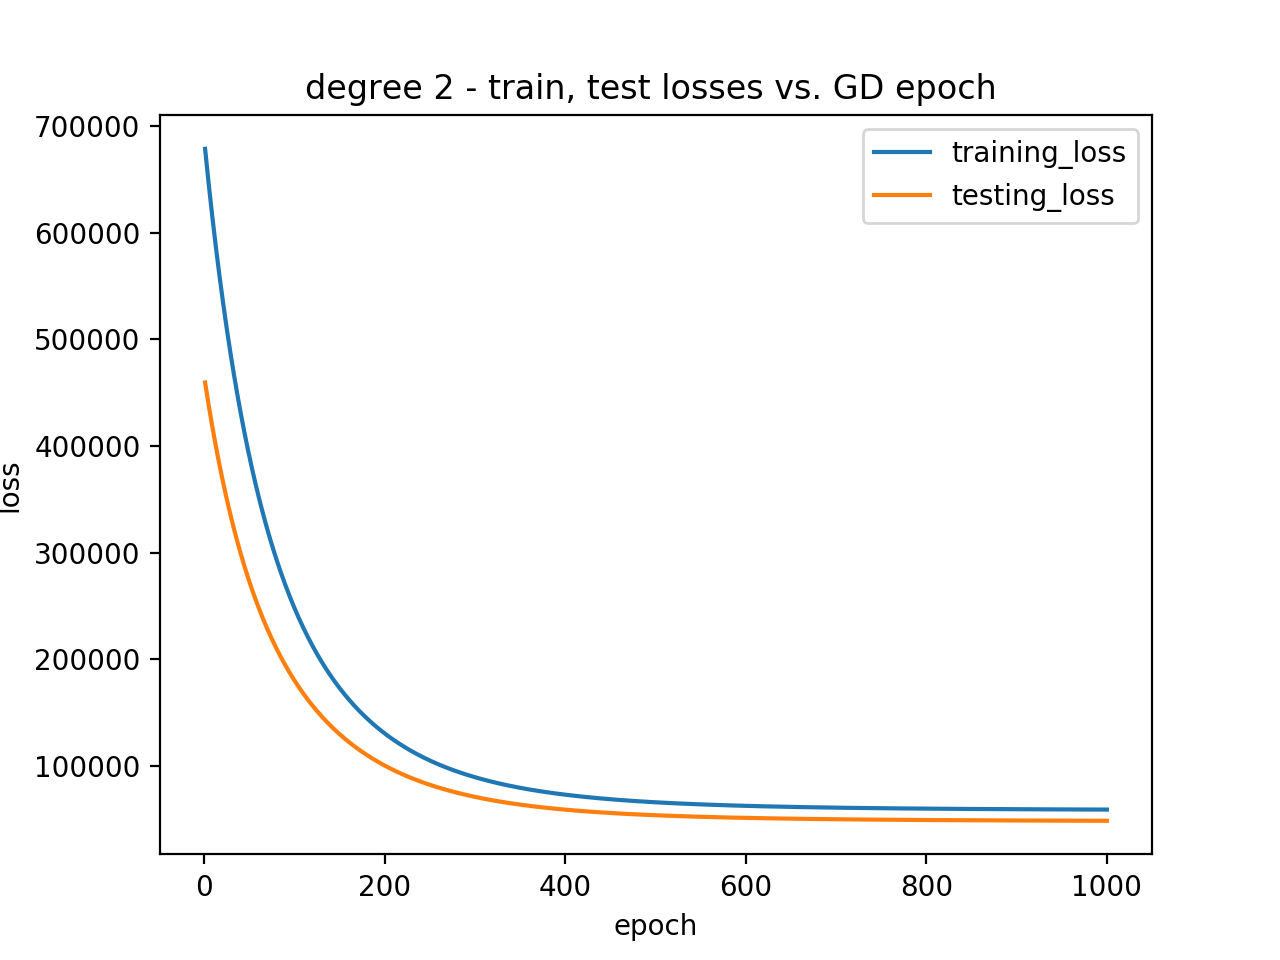
\includegraphics[width=\linewidth]{figures/d2_gd_loss.png}
    \caption{Training \& Testing Loss}
  \end{subfigure}
  \caption{Gradient Descent with Degree 2}
  \label{fig:gd_2}
\end{figure}

The plot of different example size is shown in Figure \ref{fig:example}


\begin{figure}[!h]
  \centering
  \begin{subfigure}[b]{0.4\linewidth}
    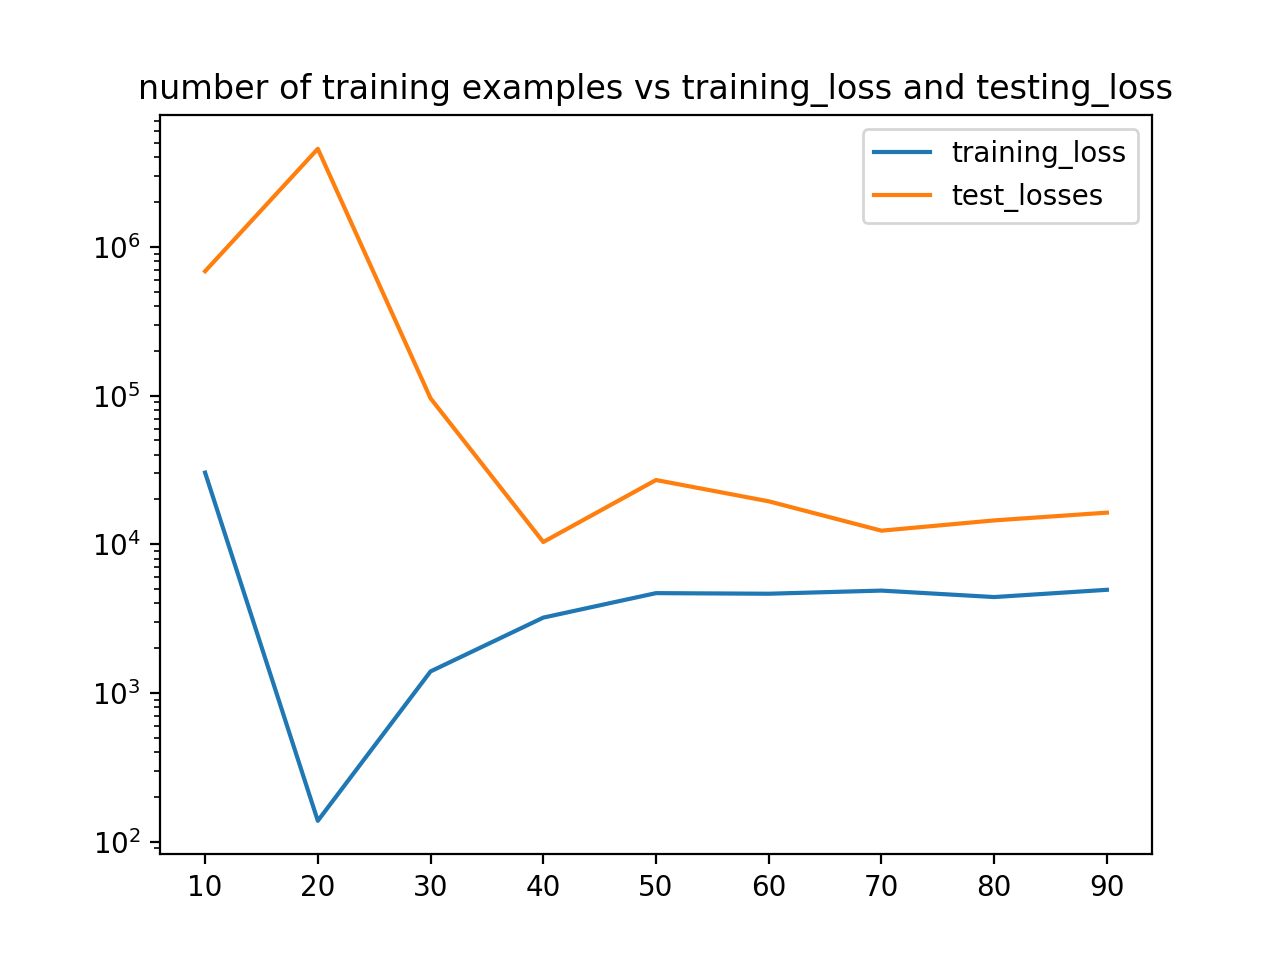
\includegraphics[width=\linewidth]{figures/example_loss.png}
  \end{subfigure}
  \caption{Loss per Example}
  \label{fig:example}
\end{figure}

\item
Ridge Regression

2.1

\medskip

2.1.1

The loss function of ridge regression equals to the sum of the linear regression loss and the coefficients' L2 norm

$$\begin{aligned}
J(\beta) &= (y - X\beta)^T(y - X\beta) + \lambda\beta^T\beta \\
&=\beta^TX^TX\beta - \beta^TX^Ty - y^TX\beta + y^Ty + \lambda\beta^T\beta \\
&=\beta^TX^TX\beta - 2\beta^TX^Ty + y^Ty + \beta^T(\lambda I)\beta
\end{aligned}$$

Get the derivative of the loss and find $\beta$ make it to $0$

$$\begin{aligned}
\nabla_{\beta}J(\beta) = \frac{\partial J(\beta)}{\partial \beta} &= 2X^TX\beta - 2X^Ty + 2(\lambda I)\beta \\
\nabla_{\beta}J(\beta) &= 0
\end{aligned}$$

$$\begin{aligned}
2X^TX\beta - 2X^Ty + 2(\lambda I)\beta = 0 \\
X^TX\beta + \lambda I\beta = X^Ty \\
\beta = (X^TX + \lambda I)^{-1} X^Ty
\end{aligned}$$

\medskip

2.1.2

No, it cannot be solve with linear regression. Use normal equation

$$\begin{aligned}
\Theta &= (X^TX)^{-1}X^Ty \\
X^TX &= \begin{bmatrix}
  35 & 70 \\
  70 & 140
\end{bmatrix} \\
|X^TX| &= 35 \times 140 - 70 \times 70 = 0
\end{aligned}$$

Because the determinant of $X^TX$ is $0$, it cannot be inverted.

2.1.3

Lasso regression, because it tends to create sparse weights.

\medskip

2.2

The training and validation loss with respect to lambda are plotted in the Figure \ref{fig:lambda_loss}. The training loss keep increasing while the lambda increasing. It makes sense because the regularization is used to generalize the model. Larger $\lambda$ menas less overfit to the training data, so the loss increases. The validation loss is in a bowl shape. With descent amount of regularization, the model is generalized well to take care of the validation data. Overly large $\lambda$ inhibits the model to learn anything, so the validation loss increases as well.

\begin{figure}[!h]
  \centering
  \begin{subfigure}[b]{0.4\linewidth}
    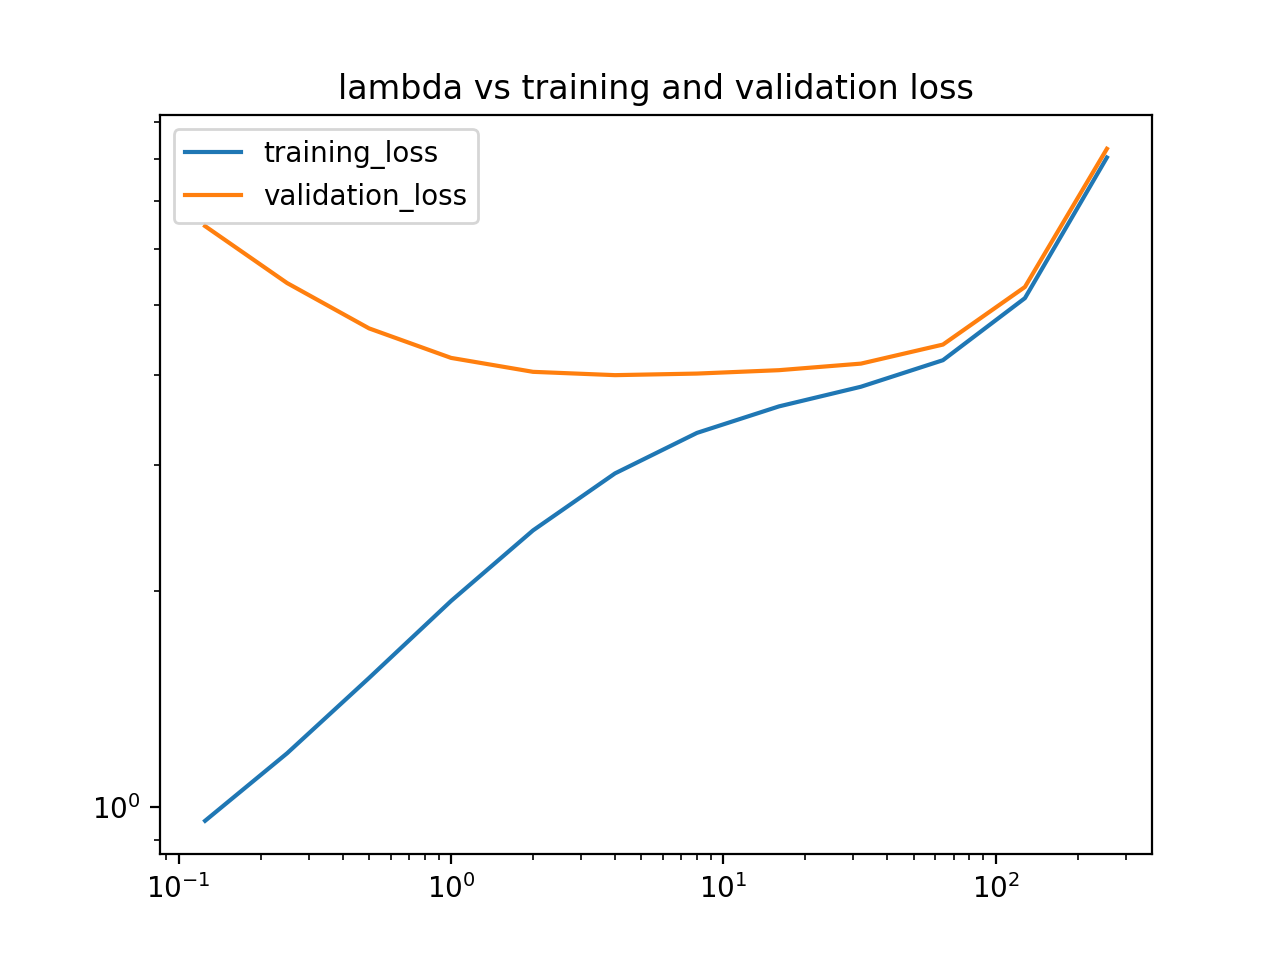
\includegraphics[width=\linewidth]{figures/lambda_loss.png}
  \end{subfigure}
  \caption{Loss per Lambda}
  \label{fig:lambda_loss}
\end{figure}

\medskip

The best $\lambda$ leaned is $4$. Its corresponding loss is $4.6368$ and the norm of $\beta$ is $6.6401$. When the $\lambda$ is $0$, the loss is $11.0313$ and the norm is $30.2697$. When the $\lambda$ is $512$, the loss is $12.1264$ and the norm is $4.6513$. The larger the $lambda$ the smaller the norm of the learned $\beta$. Overly large or small norm leads to large loss.

\medskip

The learned $\beta$ is shown in Figure \ref{fig:beta}. Comparing with the underlying distribution in the data generation, the values make sense. The second coefficient learned is indeed around $5$. The other following coefficients for noises are relatively small.

\begin{figure}[!h]
  \centering
  \begin{subfigure}[b]{0.4\linewidth}
    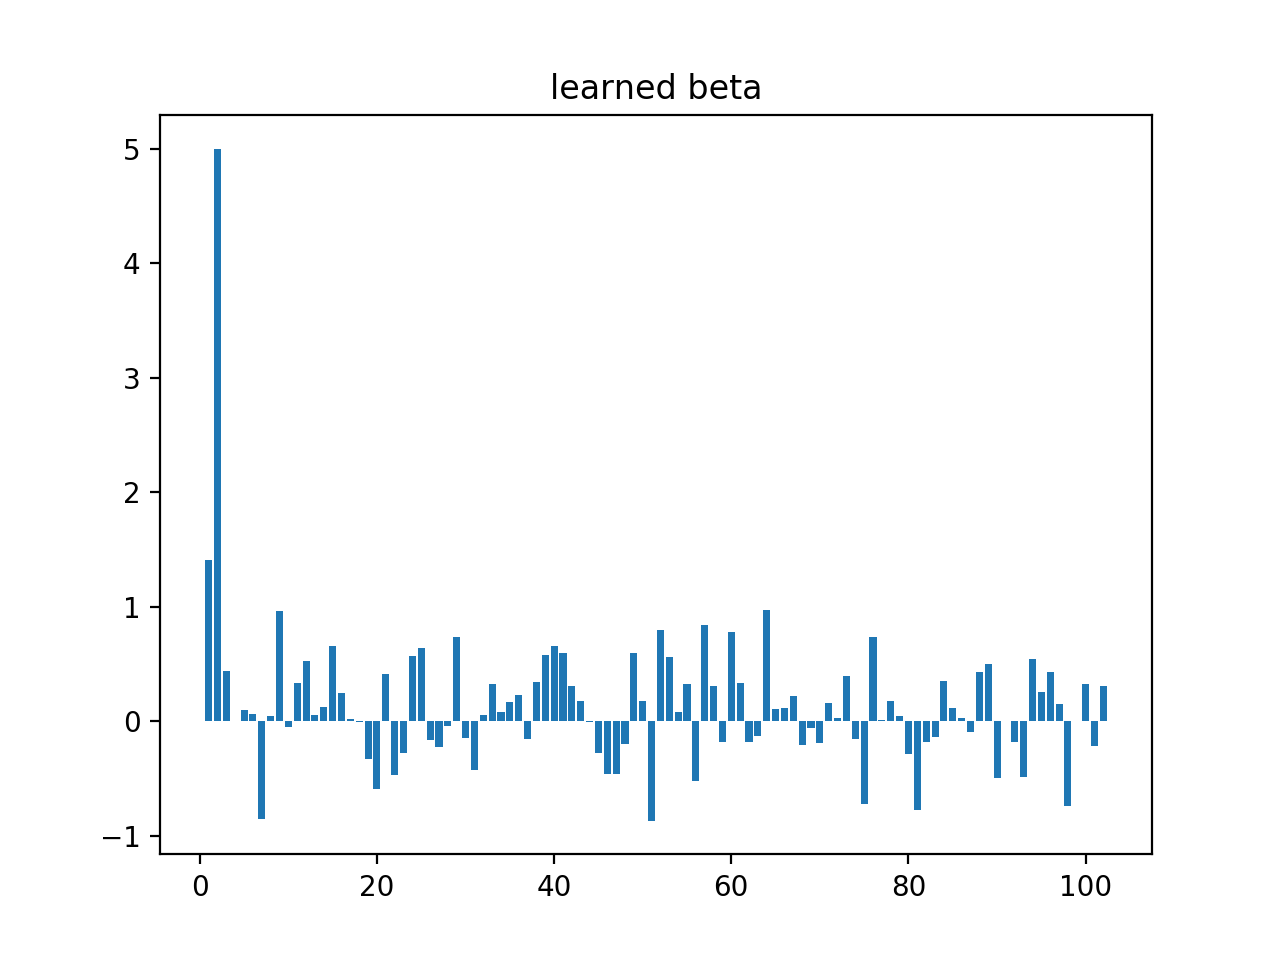
\includegraphics[width=\linewidth]{figures/beta.png}
  \end{subfigure}
  \caption{Beta}
  \label{fig:beta}
\end{figure}

\medskip

The gradient descent is also implemented for the ridge regression. The first 5 values of such learned beta is $[1.28730024,\, 5.00181111,\, 0.38442863,\, 0.04989323,\, 0.10607296]$, which closely matches the values learned in normal equation $[1.40916206,\, 5.00157608,\, 0.44139893,\, 0.00755006,\, 0.09740131]$. Moreover, the loss and the norm of the gradient descent $\beta$ are $4.6289$ and $6.2333$ which is almost the same with the ones of nomral equation reported above.

\item
Sample Questions

\medskip

3.1

It is not a good set of basis functions, because they do not overlap to cover all points. For example, when $x=4$, no matter what $\beta$ is, $y$ can only be $0$.

\medskip

3.2

The three points are $[1, 1],\, [2, 4],\, [3, 9]$.

Leave $[1,1]$ out, we have
$$
4 = 2\beta_{1} + 4\beta_{2},\;
9 = 3\beta_{1} + 9\beta_{2}
$$
$$
\beta_{1} = 0,\; \beta_{2} = 1
$$
The validation loss is $0$

Leave $[2,4]$ out, we have
$$
1 = \beta_{1} + \beta_{2},\;
9 = 3\beta_{1} + 9\beta_{2}
$$
$$
\beta_{1} = 0,\; \beta_{2} = 1
$$
The validation loss is $0$

Leave $[3,9]$ out, we have
$$
1 = \beta_{1} + \beta_{2},\;
4 = 2\beta_{1} + 4\beta_{2}
$$
$$
\beta_{1} = 0,\; \beta_{2} = 1
$$
The validation loss is $0$

So overall, the mean squared LOOCV error is $0$

% ========== Continue adding items as needed

\end{enumerate}

\end{document}
\grid
\grid
